\documentclass[11pt]{article}

\usepackage[letterpaper,top=1in,bottom=1in,left=1in,right=1in]{geometry}
\usepackage{amsmath,amsthm,amssymb}
\usepackage{graphicx}
\usepackage{hyperref}

\newtheorem{theorem}{Theorem}[section]
\newtheorem{lemma}[theorem]{Lemma}
\newtheorem{proposition}[theorem]{Proposition}
\newtheorem{corollary}[theorem]{Corollary}
\theoremstyle{definition}
\newtheorem{definition}[theorem]{Definition}
\newtheorem{example}[theorem]{Example}
\theoremstyle{remark}
\newtheorem{remark}[theorem]{Remark}
\newtheorem{conjecture}[theorem]{Conjecture}
\newtheorem{question}[theorem]{Question}

\newcommand{\R}{\mathbb{R}}
\newcommand{\N}{\mathbb{N}}
\newcommand{\bM}{\bar{\mathcal{M}}}
\newcommand{\Ha}{\mathcal{H}}
\newcommand{\ex}{\operatorname{ex}}
\newcommand{\eps}{\varepsilon}
\newcommand{\den}{\operatorname{den}}
\newcommand{\NN}{\mathcal{N}}
\newcommand{\UU}{\mathcal{U}}

\title{\textbf{Half-One Metrics and the Vertices of the Metric Body:\\
Density, Enumeration, and Angle}}

\author{David Victor Feldman\\
\small Department of Mathematics and Statistics\\
\small University of New Hampshire
\and
Eric R.\ Kehoe\\
\small Zoetis, Inc.\\
\small Fort Collins, Colorado}

\date{}

\begin{document}
\maketitle

\begin{abstract}
A half-one metric on $n$ points is a bounded-by-$1$ pseudometric taking only the values
$\tfrac12$ and $1$. Every such vector is automatically a metric, and by the criterion of
the companion paper it is an extreme point of the metric body exactly when every component
of its edge graph contains an odd cycle. We ask how much of the metric body these metrics
account for, and find that the question has three inequivalent readings with three
different kinds of answer.

Among half-one metrics themselves the answer is a theorem: the proportion that are extreme
tends to $1$, exponentially fast. Among all vertices of the metric body it is data: we
determine $|\ex(\bM_n)|$ exactly for $n\leq6$, obtaining $19$, $259$ and $27263$ with
denominator profiles, and the proportion of vertices that are half-one is not monotone.
By exterior solid angle it is a conjecture, supported here by an experiment carried far
enough to exhibit a crossover near $n=18$ that shorter ranges miss.

Along the way we correct the $q$-level feasibility density to
$P_q=\tfrac12+\tfrac1{2q^2}$, record the denominators that arise in upper-half
decompositions, and pose a bound on them that is uniform in $n$.
\end{abstract}

%%%%%%%%%%%%%%%%%%%%%%%%%%%%%%%%%%%%%%%%%%%%%%%%%%%%%%%%%%
\section{Introduction}
\label{sec:intro}
%%%%%%%%%%%%%%%%%%%%%%%%%%%%%%%%%%%%%%%%%%%%%%%%%%%%%%%%%%

Let $\bM_n$ denote the metric body: the polytope of bounded-by-$1$ pseudometrics on
$\mathbf n=\{1,\ldots,n\}$, embedded in $\R^m$ with $m=\binom n2$. Its extreme points are
the irreducible building blocks of all metrics, and identifying them is the central
difficulty of the subject \cite{Avis80,Bandelt92,Deza97,Koolen00}.

Among them the simplest after the partition metrics are the \emph{half-one metrics}.

\begin{definition}\label{def:halfone}
A \emph{half-one metric} on $n$ points is a $d\in\bM_n$ with
$d\in\{\tfrac12,1\}^{\binom n2}$. Write $\Ha_n$ for this set.
\end{definition}

Every vector in $\{\tfrac12,1\}^{\binom n2}$ is a metric, since
$d_{ij}+d_{jk}\geq\tfrac12+\tfrac12=1\geq d_{ik}$ always, so $|\Ha_n|=2^{\binom n2}$ and
half-one metrics enjoy an automatic feasibility no other denominator class has. The
companion paper \cite{FK-cone} determines which are extreme: $d\in\Ha_n$ is extreme in
$\bM_n$ if and only if every component of its edge graph $\Gamma_d$ contains an odd cycle.

This paper asks how much of $\bM_n$ the half-one metrics account for. The interest is that
the question has three readings, and they do not answer alike.

\smallskip
\noindent\textbf{(i) Among half-one metrics.} Almost all of them are extreme. This is
Theorem~\ref{thm:density}: the proportion tends to $1$, with an explicit exponential bound
on the deficit. The proof reads a random half-one metric as an Erd\H{o}s--R\'enyi graph
$G(n,\tfrac12)$ and shows that three events of high probability---an induced claw somewhere,
a local mending condition at every vertex, and connectivity---together force the edge graph
to be connected and to carry an odd cycle.

\smallskip
\noindent\textbf{(ii) Among all vertices of $\bM_n$.} Here we have data rather than a
theorem. Section~\ref{sec:census} determines $|\ex(\bM_n)|$ for $n\leq6$ by exhaustive
search over rational grids with exact rank certification:
\[
|\ex(\bM_4)|=19,\qquad |\ex(\bM_5)|=259,\qquad |\ex(\bM_6)|=27263,
\]
with the denominators occurring at $n=6$ distributed as $203$, $15090$, $7290$, $4680$ over
$1,2,3,4$. The extreme half-one metrics number $5$, $168$, $12326$, so their share of all
vertices runs $26\%$, $65\%$, $45\%$: not monotone, and the trend beyond $n=6$ is unknown.

\smallskip
\noindent\textbf{(iii) By exterior solid angle.} The probability that a given vertex
maximizes a uniformly random linear objective is proportional to the volume of its dual
cone met with the unit sphere. Section~\ref{sec:angles} reports the experiment over
$5\leq n\leq40$: partition metrics dominate through $n\approx12$, the half-one share
crosses theirs near $n=18$, and reaches $1$ by $n=40$. The Gauss--Bonnet conjecture
(Conjecture~\ref{conj:gb}) asserts that half-ones carry asymptotically all of the
exterior angle. A range stopping at $n=10$ sees none of this, which is worth recording
because such a range has been read as evidence against the trend.

\smallskip
That (i) is a theorem, (iii) a conjecture, and (ii) neither---and that (ii)'s numbers do
not obviously support (iii)---is the shape of the subject as we find it.

Sections~\ref{sec:denominators} and~\ref{sec:qlevel} treat the complement of the question:
what the vertices that are \emph{not} half-one look like, and why they are scarce.
Section~\ref{sec:denominators} records the denominators arising in decompositions of the
upper half of $\bM_n$ and conjectures a bound on them uniform in $n$;
Section~\ref{sec:qlevel} computes the density of $q$-level points that are metrics,
corrects that density to $P_q=\tfrac12+\tfrac1{2q^2}$, and derives the vanishing of
$\operatorname{Vol}(\bM_n)$.

Throughout, computations are exact unless stated otherwise; the paper, the formalization,
and every script behind the tables are archived at
\href{https://doi.org/10.5281/zenodo.21953234}{doi:10.5281/zenodo.21953234}
(GitHub: \texttt{DavidVFeldman/half-one-metrics}).

Much of the paper is formally verified. A Lean~4 development accompanying this article
(\texttt{HalfOne}, in the archive above) proves, over $\mathbb Q$ and from a
perturbation-form definition of extremality: the perturbation lemma
(Lemma~\ref{lem:pert}), Proposition~\ref{prop:onedegen},
Theorem~\ref{thm:upperhalf} and Corollary~\ref{cor:valuesets}, the twin characterization and the
Bonferroni bound of Theorem~\ref{thm:twinbound} as an exact cardinality inequality, the
counting identity behind Proposition~\ref{prop:Pq}, Proposition~\ref{prop:descent}, and,
for Theorem~\ref{thm:density}, both its deterministic core (connectivity, mending and a
claw force the criterion) and the three counting bounds of its proof, assembled into the
finite-$n$ deficit inequality. The census counts of $|\ex(\Ha_n)|$ are theorems of the
development for $n\leq7$: a checker is proved equivalent to the bipartite-component
criterion and then executed inside the proof assistant, by kernel reduction for $n\leq5$
and by the compiled evaluator (Lean's \texttt{native\_decide}, which enlarges the trusted
base by the compiler) for $n=6,7$. The criterion itself
(Theorem~\ref{thm:criterion}) is the companion paper's theorem and is quoted, not
reproved: the formal census counts graphs satisfying the combinatorial predicate. One
observation surfaced by the formalization is worth recording: in
Proposition~\ref{prop:descent}, positive definiteness is not needed for the pullback
direction---the pullback of any vertex along any quotient map is a vertex, the zero
coordinates pinning every perturbation to a pullback; positive definiteness is what makes
the descent canonical.

%%%%%%%%%%%%%%%%%%%%%%%%%%%%%%%%%%%%%%%%%%%%%%%%%%%%%%%%%%
\section{Preliminaries}
\label{sec:prelim}
%%%%%%%%%%%%%%%%%%%%%%%%%%%%%%%%%%%%%%%%%%%%%%%%%%%%%%%%%%

We follow \cite{FK-cone}. For $d\in\bM_n$ write $\UU_d=\{E:d_E=1\}$ for the unital edges
and $\NN_d$ for the rest. A triangle is \emph{degenerate} when one of its
sides equals the sum of the other two. The \emph{edge graph} $\Gamma_d$ has node set
$\NN_d$, with $E$ and $E'$ adjacent when they are the two short sides of a degenerate
triangle.

A point of $\bM_n$ is extreme exactly when it is the unique metric satisfying its tight
constraints, so extremality is detected by \emph{perturbations}: symmetric $\eps$ vanishing
on the diagonal with $d\pm\eps\in\bM_n$. Two facts about them are used constantly, and we
record their one-line proofs rather than import them.

\begin{lemma}\label{lem:pert}
Let $\eps$ be a perturbation at $d\in\bM_n$. Then
\begin{enumerate}
\item[(i)] $|\eps_E|\leq\min\{d_E,1-d_E\}$ for every $E$; in particular $\eps$ vanishes
wherever $d$ is $0$ or $1$.
\item[(ii)] If the triangle on $i,j,k$ is degenerate at $d$, say $d_{ik}=d_{ij}+d_{jk}$,
then $\eps_{ik}=\eps_{ij}+\eps_{jk}$.
\end{enumerate}
\end{lemma}

\begin{proof}
(i) $d\pm\eps\in\bM_n$ forces $0\leq d_E\pm\eps_E\leq1$. (ii) The triangle inequality for
$d+\eps$ gives $\eps_{ik}\leq\eps_{ij}+\eps_{jk}$ and for $d-\eps$ the reverse.
\end{proof}

For a half-one metric the situation is especially simple, because $\tfrac12+\tfrac12=1$ is
the only degeneracy available.

\begin{proposition}\label{prop:onedegen}
A strictly positive $d\in\bM_n$ has at most one degenerate ordered triangle on any given
triple of points.
\end{proposition}

\begin{proof}
Suppose $d_{ik}=d_{ij}+d_{jk}$ and $d_{ij}=d_{ik}+d_{kj}$. Adding gives
$d_{jk}+d_{kj}=0$, so $d_{jk}=0$.
\end{proof}

\begin{proposition}\label{prop:halfonegamma}
Let $d\in\Ha_n$ and let $G_d$ be the graph on $\mathbf n$ whose edges are the half-length
pairs. Then $\{i,j\}$ and $\{i,k\}$ are adjacent in $\Gamma_d$ if and only if both are
edges of $G_d$ and $\{j,k\}$ is not.
\end{proposition}

\begin{proof}
A degenerate triangle of a half-one metric has $\tfrac12+\tfrac12=1$, so its two short
sides are half-length and its long side unital. Conversely two half-length sides meeting at
$i$ with unital third side form such a triangle.
\end{proof}

So $\Gamma_d$ is obtained from the line graph of $G_d$ by deleting the adjacencies that
come from triangles of $G_d$. We quote the criterion.

\begin{theorem}[\cite{FK-cone}]\label{thm:criterion}
$d\in\Ha_n$ is extreme in $\bM_n$ if and only if every component of $\Gamma_d$ contains an
odd cycle. Equivalently, no component of $\Gamma_d$ is bipartite; isolated nodes count as
components.
\end{theorem}

%%%%%%%%%%%%%%%%%%%%%%%%%%%%%%%%%%%%%%%%%%%%%%%%%%%%%%%%%%
\section{Almost every half-one metric is extreme}
\label{sec:density}
%%%%%%%%%%%%%%%%%%%%%%%%%%%%%%%%%%%%%%%%%%%%%%%%%%%%%%%%%%

Identifying $d\in\Ha_n$ with its half-length graph $G_d$ makes the uniform distribution on
$\Ha_n$ the Erd\H{o}s--R\'enyi distribution $G(n,\tfrac12)$.

\begin{theorem}\label{thm:density}
Let $d$ be a uniformly random half-one metric on $n$ points. Then
\[
\Pr\bigl[d\notin\ex(\Ha_n)\bigr]\;\leq\;
\Bigl(\tfrac{15}{16}\Bigr)^{\lfloor n/4\rfloor}
+\tfrac{n^3}{2}\Bigl(\tfrac78\Bigr)^{n-3}
+\sum_{k=1}^{\lfloor n/2\rfloor}\binom nk 2^{-k(n-k)} ,
\]
and in particular
\[
\lim_{n\to\infty}\frac{|\ex(\Ha_n)|}{2^{\binom n2}}=1 .
\]
\end{theorem}

\begin{proof}
Write $G=G_d$. By Theorem~\ref{thm:criterion} it suffices to exhibit events forcing
$\Gamma_d$ to be connected and to contain an odd cycle.

\emph{An odd cycle.} Suppose $G$ contains an induced claw: a vertex $i$ with neighbours
$j,k,l$ pairwise non-adjacent. By Proposition~\ref{prop:halfonegamma} the three nodes
$\{i,j\},\{i,k\},\{i,l\}$ are pairwise adjacent in $\Gamma_d$, a triangle. To bound the
probability that no induced claw exists, partition $\mathbf n$ into $\lfloor n/4\rfloor$
disjoint $4$-sets. A fixed $4$-set spans an induced claw with probability
$4\cdot2^{-6}=\tfrac1{16}$: six pairs are prescribed, and the four choices of centre give
disjoint events. Distinct $4$-sets involve disjoint pairs, hence independent events, and
the first term follows.

\emph{Local mending.} Call $i$ \emph{mended} when for all $j,k\in N_G(i)$ the nodes
$\{i,j\}$ and $\{i,k\}$ lie in a common component of $\Gamma_d$. If $\{j,k\}\notin G$ they
are adjacent outright. If $\{j,k\}\in G$, any $l\notin\{i,j,k\}$ with
\[
\{i,l\}\in G,\qquad \{j,l\}\notin G,\qquad\{k,l\}\notin G
\]
supplies the path $\{i,j\}\sim\{i,l\}\sim\{i,k\}$. For a fixed triple these three
conditions hold for a given $l$ with probability $\tfrac18$, independently over the $n-3$
candidates and of the pairs inside $\{i,j,k\}$. There are at most $n\binom{n-1}2\leq n^3/2$
triples, giving the second term.

\emph{Connectivity.} The third term is the standard union bound on
$\Pr[G\text{ disconnected}]$ over vertex subsets spanning no crossing pair.

Suppose all three events hold. Any two edges of the connected graph $G$ are joined by a
walk in which consecutive edges share a vertex, and consecutive edges at a mended vertex
lie in a common component of $\Gamma_d$; hence $\Gamma_d$ is connected. It contains the
triangle furnished by the claw, so by Theorem~\ref{thm:criterion} $d$ is extreme.
\end{proof}

\begin{remark}\label{rem:notsharp}
The bound is far from sharp; it is a limit statement whose constants bite only for large
$n$. Exhaustive enumeration gives
\begin{center}
\begin{tabular}{r|r|r|r}
$n$ & $2^{\binom n2}$ & $|\ex(\Ha_n)|$ & proportion\\
\hline
$4$ & $64$ & $5$ & $0.0781$\\
$5$ & $1024$ & $168$ & $0.1641$\\
$6$ & $32768$ & $12326$ & $0.3762$\\
$7$ & $2097152$ & $1309868$ & $0.6246$\\
$8$ & $268435456$ & $209717144$ & $0.7813$
\end{tabular}
\end{center}
and sampling puts the proportion above $0.99$ already at $n=15$, where it reads $0.9937$
against $0.9889$ at $n=14$. How far from sharp the bound is can be said exactly: the
right-hand side of Theorem~\ref{thm:density} exceeds $1$, and so says nothing, for every
$n\leq103$, the term $\tfrac{n^3}2(\tfrac78)^{n-3}$ dominating until about $n=150$ and
$(\tfrac{15}{16})^{\lfloor n/4\rfloor}$ thereafter. The theorem is a limit statement, and
the range in which anything is computable lies entirely inside the range where its explicit
bound is vacuous. The deficit is examined next, and its leading term identified.
\end{remark}

The commonest single obstruction to extremality is an isolated node of $\Gamma_d$, and it
has a graph-theoretic name.

\begin{proposition}\label{prop:twins}
For $d\in\Ha_n$, an edge $\{i,j\}$ of $G_d$ is an isolated node of $\Gamma_d$ if and only
if $i$ and $j$ are \emph{true twins} in $G_d$: adjacent, with identical neighbourhoods
elsewhere.
\end{proposition}

\begin{proof}
By Proposition~\ref{prop:halfonegamma} the node $\{i,j\}$ acquires a neighbour at $k$
exactly when one of $\{i,k\},\{j,k\}$ lies in $G_d$ and the other does not.
\end{proof}

An isolated node is a bipartite component, so a true twin pair certifies non-extremality,
and counting twin pairs bounds the deficit from below.

\begin{theorem}\label{thm:twinbound}
\[
1-\frac{|\ex(\Ha_n)|}{2^{\binom n2}}\;\geq\;
\binom n2\,2^{-(n-1)}\Bigl(1-O\bigl(n^2 2^{-n}\bigr)\Bigr).
\]
\end{theorem}

\begin{proof}
For a pair $\{i,j\}$ let $A_{ij}$ be the event that $i,j$ are true twins in
$G\sim G(n,\tfrac12)$: the pair $\{i,j\}$ is present, and for each of the $n-2$ remaining
vertices $k$ the pairs $\{i,k\}$ and $\{j,k\}$ agree. These are $n-1$ independent fair
events, so $\Pr[A_{ij}]=2^{-(n-1)}$.

For the second Bonferroni term, two cases. If the pairs share a vertex, say $A_{ij}$ and
$A_{ik}$: the twin condition of $\{i,j\}$ applied at $k$ forces $\{j,k\}\in G$, so all
three pairs among $i,j,k$ are present, and for each of the $n-3$ outside vertices $x$ the
three pairs $\{i,x\},\{j,x\},\{k,x\}$ agree; hence
$\Pr[A_{ij}\cap A_{ik}]=2^{-3}\cdot2^{-2(n-3)}=2^{-(2n-3)}$. If the pairs are disjoint,
$A_{ij}$ and $A_{kl}$: the pairs $\{i,j\}$ and $\{k,l\}$ are present, each of the $n-4$
outside vertices contributes two agreements, and on the four pairs between $\{i,j\}$ and
$\{k,l\}$ the two twin conditions force all four to agree, leaving one free bit of four;
hence $\Pr[A_{ij}\cap A_{kl}]=2^{-2}\cdot2^{-2(n-4)}\cdot2^{-3}=2^{-(2n-3)}$. Both
formulas were confirmed by direct enumeration at $n=5$.

There are fewer than $n^4/8$ unordered pairs of distinct pairs, so by Bonferroni
\[
\Pr\Bigl[\bigcup A_{ij}\Bigr]\;\geq\;\binom n2 2^{-(n-1)}-\tfrac{n^4}8\,2^{-(2n-3)}
\;=\;\binom n2 2^{-(n-1)}\Bigl(1-O\bigl(n^22^{-n}\bigr)\Bigr).\qedhere
\]
\end{proof}

Exhaustive classification of every non-extreme half-one metric through $n=8$ shows the twin
obstruction becoming dominant:

\begin{center}
\begin{tabular}{r|r|r|r|r}
$n$ & non-extreme & with a twin pair & other & twin share\\
\hline
$4$ & $59$ & $32$ & $27$ & $0.54$\\
$5$ & $856$ & $436$ & $420$ & $0.51$\\
$6$ & $20442$ & $11292$ & $9150$ & $0.55$\\
$7$ & $787284$ & $545784$ & $241500$ & $0.69$\\
$8$ & $58718312$ & $49826744$ & $8891568$ & $0.85$
\end{tabular}
\end{center}

Among the remainder the smallest bipartite component most often has two nodes, an event of
probability $O(n^3 4^{-n})$ per configuration, and every mode observed decays at least this
fast against the twin rate. Accordingly:

\begin{conjecture}\label{conj:deficit}
$\displaystyle 1-\frac{|\ex(\Ha_n)|}{2^{\binom n2}}\;\sim\;\binom n2\,2^{-(n-1)}$ as
$n\to\infty$.
\end{conjecture}

Writing $D_n$ for the deficit and $\lambda_n=\binom n2 2^{-(n-1)}$ for the twin rate, the
conjecture asserts $D_n/\lambda_n\to1$. That ratio is not monotone: it rises, crosses $1$
near $n=8$, and returns to $1$ from below.

\begin{center}
\begin{tabular}{r|r|r|r|l}
$n$ & $D_n$ & $\lambda_n$ & $D_n/\lambda_n$ & warrant\\
\hline
$4$ & $0.921875$ & $0.750000$ & $1.2292$ & exact\\
$5$ & $0.835938$ & $0.625000$ & $1.3375$ & exact\\
$6$ & $0.623840$ & $0.468750$ & $1.3309$ & exact\\
$7$ & $0.375406$ & $0.328125$ & $1.1441$ & exact\\
$8$ & $0.218743$ & $0.218750$ & $1.0000$ & exact\\
$9$ & $0.134295$ & $0.140625$ & $0.9550$ & sampled\\
$10$ & $0.084368$ & $0.087891$ & $0.9599$ & sampled\\
$11$ & $0.052074$ & $0.053711$ & $0.9695$ & sampled\\
$12$ & $0.031611$ & $0.032227$ & $0.9809$ & sampled\\
$13$ & $0.018767$ & $0.019043$ & $0.9855$ & sampled\\
$14$ & $0.011060$ & $0.011108$ & $0.9956$ & sampled\\
$15$ & $0.006339$ & $0.006409$ & $0.9891$ & sampled\\
$16$ & $0.003653$ & $0.003662$ & $0.9974$ & sampled
\end{tabular}
\end{center}

The sampled rows use $3\times10^6$ draws each, giving a standard error on the ratio that
runs from $0.0014$ at $n=9$ to $0.0095$ at $n=16$; the estimator was checked against the
exact values at $n=6,7,8$. Every sampled row lies above the floor
$1-\tfrac{n^4}8 2^{-(2n-3)}/\lambda_n$ guaranteed by Theorem~\ref{thm:twinbound}, which is
the one consistency check the data owe the proof. The agreement at $n=8$ is a crossing and
not an identity; the two columns are equal there to five decimal places by coincidence.

\begin{remark}\label{rem:illusion}
The deficit was previously observed to fit $c\,(0.6)^n$ over the computable range, a rate
matching no candidate obstruction. The mystery is an artifact of fitting a pure exponential
to a sequence with a polynomial factor. Fit $\lambda_n=\binom n2 2^{-(n-1)}$ itself: the
geometric mean of successive ratios over $4\leq n\leq17$ is $0.636$, and over
$8\leq n\leq17$ it is $0.596$; log-linear least squares on the same ranges returns $0.627$
and $0.594$. Every one of these is an apparent base near $0.6$ for a sequence whose actual
base is $\tfrac12$. The observed $0.6$ is the twin law in disguise.
\end{remark}

\begin{remark}\label{rem:starcomplement}
The proof can be recast, with a better rate, by observing that the nodes
$\{\{i,x\}:x\in N_G(i)\}$ induce in $\Gamma_d$ exactly the \emph{complement} of
$G[N_G(i)]$: two spokes at $i$ are adjacent precisely when the connecting pair is unital.
Conditioned on $N_G(i)$ that complement is again $G(\deg i,\tfrac12)$, and $\deg i\geq n/3$
holds for all $i$ with probability $1-e^{-\Omega(n)}$. An induced claw at $i$ is a triangle
in that complement.
\end{remark}

Theorem~\ref{thm:density} settles \cite[Conjecture 4.1.4]{Kehoe19}, whose printed statement
asserts $|\Ha_n|\sim2^{\binom n2}$ and is to be read with $\ex(\Ha_n)$ in place of $\Ha_n$:
the former is an identity, every element of $\{\tfrac12,1\}^{\binom n2}$ being a metric. It
also subsumes the earlier counting bounds. Cayley's formula and Proposition~\ref{prop:tree}
below give $|\ex(\Ha_n)|>n^{n-2}-\tfrac{n!}2$, of order $2^{n\log n}$; the truth is
$(1-o(1))2^{\binom n2}$.

\begin{proposition}\label{prop:tree}
If $G_d$ is a spanning tree that is not a path, then $d$ is extreme. More generally, if
$G_d$ is triangle-free and every component has a vertex of degree at least $3$, then $d$ is
extreme.
\end{proposition}

\begin{proof}
A triangle-free $G_d$ has $\Gamma_d$ equal to the line graph of $G_d$ by
Proposition~\ref{prop:halfonegamma}, and the line graph of a connected graph is connected,
so the components of $\Gamma_d$ correspond to those of $G_d$. A vertex of degree $3$
contributes a triangle to the line graph. Apply Theorem~\ref{thm:criterion}.
\end{proof}

\begin{remark}
The resulting inequality is strict at every $n$, since the all-unital metric $d\equiv1$ is
extreme and is counted by no spanning tree; at $n=4$ it is the only extreme half-one beyond
the four stars, so $|\ex(\Ha_4)|=5$ against $n^{n-2}-\tfrac{n!}2=4$. Comparison with the
Bell numbers $B_n$, which count the partition metrics, gives $|\ex(\Ha_n)|>B_n$ for all
$n\geq5$ by the bound of Berend and Tassa \cite{Berend10};
at $n=4$ the inequality fails, $5<15$.
\end{remark}

The half-one metrics are not merely a convenient family; two results locate them exactly.
The first is a corollary of the cube identity of \cite{FK-cone} rather than a new fact about
$\bM_n$, but it is not stated there and is used repeatedly below.

\begin{theorem}\label{thm:upperhalf}
Every extreme point of $\bM_n$ all of whose distances are at least $\tfrac12$ is a half-one
metric:
\[
\ex(\bM_n)\cap[\tfrac12,1]^{\binom n2}\;=\;\ex(\Ha_n).
\]
\end{theorem}

\begin{proof}
The companion paper shows $\bM_n\cap[\tfrac12,1]^{\binom n2}=[\tfrac12,1]^{\binom n2}$: any
vector with all entries at least $\tfrac12$ satisfies every triangle inequality, since two
sides sum to at least $1$. An extreme point of $\bM_n$ lying in a convex subset of $\bM_n$
is extreme in that subset, so a vertex of $\bM_n$ in the upper half is a vertex of the cube,
that is, a point of $\{\tfrac12,1\}^{\binom n2}=\Ha_n$. The reverse containment is trivial.

The following direct argument avoids the cube identity and locates the failure. Let $d$ be
extreme with all values in $[\tfrac12,1]$ and suppose some value $v=d_E\in(\tfrac12,1)$. The
coordinate $E$ then lies in no tight constraint of $\bM_n$ at $d$: not in a bound, since
$0<v<1$; not as the long side of a degenerate triangle, since the two short sides sum to at
least $1>v$; and not as a short side, since then the long side would be
$v+z\geq v+\tfrac12>1$. Every constraint involving $E$ being slack, the coordinate
perturbation $\pm\delta e_E$ preserves membership in $\bM_n$ for small $\delta>0$,
contradicting extremality.
\end{proof}

So the vertex set of the upper half-cube of \cite{FK-cone} is completely determined, and
every vertex of $\bM_n$ beyond the half-one family has some distance strictly below
$\tfrac12$---as the census of the next section will exhibit in quantity.

\begin{corollary}[why half and one]\label{cor:valuesets}
Let $V\subseteq(0,1]$ satisfy $2\inf V\geq\sup V$, so that every vector in
$V^{\binom n2}$ is a metric. Then
\[
\ex(\bM_n)\cap V^{\binom n2}\;=\;\ex(\Ha_n)\cap V^{\binom n2}.
\]
In particular the intersection is empty if $1\notin V$, equals $\{d\equiv1\}$ if $1\in V$
but $\tfrac12\notin V$, and $\{\tfrac12,1\}$ is the only automatically feasible value set
yielding anything more.
\end{corollary}

\begin{proof}
Let $d\in V^{\binom n2}$ be extreme and let $M$ be its largest value. If $M<1$ then the
scaling perturbation $\pm\delta d$ preserves $\bM_n$ for small $\delta$: bounds have slack,
and the triangle constraints are homogeneous; so $d$ is not extreme. Hence $M=1$, so
$\sup V=1$ and the hypothesis puts $V\subseteq[\tfrac12,1]$, and
Theorem~\ref{thm:upperhalf} applies. For the last clause: the value sets $\{\tfrac1k,1\}$
with $k\geq3$ are excluded by the hypothesis, and genuinely fail it, the vector with one
unital pair and the rest $\tfrac1k$ violating the triangle inequality already at $n=3$.
\end{proof}

%%%%%%%%%%%%%%%%%%%%%%%%%%%%%%%%%%%%%%%%%%%%%%%%%%%%%%%%%%
\section{The vertices of $\bM_n$ for small $n$}
\label{sec:census}
%%%%%%%%%%%%%%%%%%%%%%%%%%%%%%%%%%%%%%%%%%%%%%%%%%%%%%%%%%

A vertex of $\bM_n$ is a rational point, being the unique solution of a rational linear
system, and its denominator is bounded. One may therefore enumerate the vertices of
denominator dividing $L$ exhaustively: run over $\{0,\tfrac1L,\ldots,1\}^m$ with the
triangle inequalities used to prune, and certify each surviving point by computing the rank
of its tight constraint system. Taking $L$ through the denominators that occur settles
$|\ex(\bM_n)|$.

\begin{theorem}\label{thm:census}
$|\ex(\bM_4)|=19$, $|\ex(\bM_5)|=259$ and $|\ex(\bM_6)|=27263$. The denominators occurring
are $\{1,2\}$ for $n\leq5$ and $\{1,2,3,4\}$ for $n=6$, with multiplicities
\[
\begin{array}{r|rrrr}
\den & 1 & 2 & 3 & 4\\\hline
n=6 & 203 & 15090 & 7290 & 4680
\end{array}
\]
\end{theorem}

The four sweeps cross-check: at $n=6$ the grids $L=2,3,4$ return $15293$, $7493$ and
$19973$ vertices, which are the cumulative sums $203+15090$, $203+7290$ and
$203+15090+4680$ of the table. At $n=5$ the $L=4$ sweep returns the same $259$ as $L=2$,
confirming that no vertex of denominator $3$ or $4$ is missed there, and at $n=4$ the $L=6$
sweep returns the same $19$ as $L=2$.

\begin{proposition}\label{prop:pd}
The positive-definite vertices of $\bM_n$ of denominator dividing $2$ are exactly the
extreme half-one metrics.
\end{proposition}

\begin{proof}
A vertex of denominator dividing $2$ takes values in $\{0,\tfrac12,1\}$, and is positive
definite exactly when the value $0$ is unused, that is, when it lies in
$\{\tfrac12,1\}^{\binom n2}=\Ha_n$.
\end{proof}

Accordingly the census returns $5$, $168$ and $12326$ positive-definite denominator-$2$
vertices for $n=4,5,6$, matching the enumeration of Remark~\ref{rem:notsharp} exactly and
by an independent route.

The vertices that are not positive definite are accounted for by the positive-definite ones
on fewer points, so the census reduces to a single sequence.

\begin{proposition}\label{prop:descent}
Write $\pi_d$ for the partition of $\mathbf n$ induced by $d_{xy}=0$ and $\operatorname{pd}(k)$
for the number of positive-definite vertices of $\bM_k$. Then $d$ is a vertex of $\bM_n$ if
and only if the induced metric on the quotient $\mathbf n/\pi_d$ is a positive-definite
vertex there, and consequently
\[
|\ex(\bM_n)|=\sum_{k=1}^{n}S(n,k)\operatorname{pd}(k),
\]
$S(n,k)$ the Stirling numbers of the second kind.
\end{proposition}

\begin{proof}
A perturbation $\eps$ at $d$ satisfies $|\eps|\leq\min\{d,1-d\}$ by
Lemma~\ref{lem:pert}(i), so it vanishes on every
pair inside a block of $\pi_d$. If $x,x'$ lie in one block and $y$ in another, the triangle
on $x,x',y$ is degenerate, so additivity gives $\eps_{xy}=\eps_{xx'}+\eps_{x'y}=\eps_{x'y}$:
the perturbation is constant on blocks and descends. Perturbations of $d$ and of the induced
quotient metric therefore correspond, and extremality is preserved in both directions.
Summing over the $S(n,k)$ partitions with $k$ blocks gives the count.
\end{proof}

So $\operatorname{pd}(1)=\operatorname{pd}(2)=\operatorname{pd}(3)=1$,
$\operatorname{pd}(4)=5$, $\operatorname{pd}(5)=168$, $\operatorname{pd}(6)=24296$, and
Theorem~\ref{thm:census} is recovered as $1+7+6+5=19$, $1+15+25+50+168=259$ and
$1+31+90+325+2520+24296=27263$. This furnishes a check on the census independent of the
sweeps: the $68$ orbit representatives of the positive-definite vertices of $\bM_6$
tabulated in \cite[\S5.1]{Kehoe19} expand to $24296$ points under $S_6$, and the identity
above then returns $27263$, so no orbit is missing from that table and none is redundant.
The same expansion splits the denominator-$2$ column of Theorem~\ref{thm:census} as
$15090=12325+65\cdot4+15\cdot167$, the last two terms being the denominator-$2$ vertices
carried up from $\bM_4$ and $\bM_5$, and identifies the denominator-$1$ column as the
partition metrics, $203=B_6$.

Comparing the two counts answers reading (ii) of the introduction:

\begin{center}
\begin{tabular}{r|r|r|r}
$n$ & $|\ex(\bM_n)|$ & $|\ex(\Ha_n)|$ & share\\
\hline
$4$ & $19$ & $5$ & $0.263$\\
$5$ & $259$ & $168$ & $0.649$\\
$6$ & $27263$ & $12326$ & $0.452$
\end{tabular}
\end{center}

What is known about the growth of $|\ex(\bM_n)|$ brackets it between two exponents.

\begin{proposition}\label{prop:ubt}
\[
\bigl(1-o(1)\bigr)\binom n2\;\leq\;\log_2|\ex(\bM_n)|\;\leq\;
\Bigl(\tfrac12+o(1)\Bigr)\binom n2\log_2 n .
\]
\end{proposition}

\begin{proof}
The lower bound is Theorem~\ref{thm:density}. For the upper bound, $\bM_n$ is an
$m$-polytope, $m=\binom n2$, with at most $3\binom n3+\binom n2=(n-1)\binom n2$ facets:
the triangle inequalities and the caps $d_E\leq1$, the bounds $d_E\geq0$ being implied by
sums of triangle inequalities for $n\geq3$. By the upper bound theorem of McMullen
\cite{McMullen70}, an $m$-polytope with $N$ facets has at most
$\binom{N-\lceil m/2\rceil}{\lfloor m/2\rfloor}
+\binom{N-\lfloor m/2\rfloor-1}{\lceil m/2\rceil-1}\leq2\binom{N}{\lfloor m/2\rfloor}$
vertices, and $\binom Nk\leq(eN/k)^k$ with $N=(n-1)m$ and $k=\lfloor m/2\rfloor$ gives
$\log_2|\ex(\bM_n)|\leq\tfrac m2\log_2 n\,(1+o(1))$.
\end{proof}

At $n=6$ the asymptotic expressions evaluate to $15$ and $19.4$, while
$\log_2 27263\approx14.73$ sits below both: the $o(1)$ corrections still dominate at this
size, and the count has not yet chosen between the exponents.

\begin{question}\label{q:share}
Does $|\ex(\Ha_n)|/|\ex(\bM_n)|$ tend to a limit, and if so to what? The three available
values are not monotone. Since $|\ex(\Ha_n)|=(1-o(1))2^{\binom n2}$ by
Theorem~\ref{thm:density}, the share tends to a positive limit or to zero according as
$\log_2|\ex(\bM_n)|-\binom n2$ stays bounded or tends to infinity, and by
Proposition~\ref{prop:ubt} either remains possible: the question is whether the logarithmic
factor in the upper bound is real.
\end{question}

Question~\ref{q:share} is the point at which readings (ii) and (iii) may part company: the
half-one metrics could carry asymptotically all of the exterior angle while forming a
vanishing fraction of the vertices, if the remaining vertices proliferate with small angles.
Nothing in our data excludes this, and nothing supports it.

%%%%%%%%%%%%%%%%%%%%%%%%%%%%%%%%%%%%%%%%%%%%%%%%%%%%%%%%%%
\section{Which denominators occur}
\label{sec:denominators}
%%%%%%%%%%%%%%%%%%%%%%%%%%%%%%%%%%%%%%%%%%%%%%%%%%%%%%%%%%

Beyond $n=6$ the census is out of reach, but the denominators may be sampled. Solving
$10^3$ random linear objectives over $\bM_n$ and rationalizing the optima exactly gives
denominator sets $\{1,2\}$ for $n\leq5$, $\{1,2,3,4\}$ at $n=6$, $\{1,\ldots,6\}$ at $n=7$
and $\{1,\ldots,7\}$ at $n=8$, in agreement with Theorem~\ref{thm:census} where both apply.

A second question concerns not which denominators exist but which are needed. Write
$\bM_n^{\geq1/2}=\bM_n\cap[\tfrac12,1]^m$ for the upper half of the body; by
\cite{FK-cone} this is exactly the cube $[\tfrac12,1]^m$, every point of which is a convex
combination of at most $m+1$ half-one metrics, and every half-one metric is in turn a convex
combination of vertices of the minimal face containing it. Carrying out the second step by
repeated bisection of that face---at the current point take a direction in the lineality
space of its smallest face, walk to both boundaries, split, recurse---produces a
decomposition whose leaves are vertices of $\bM_n$.

Each bisection multiplies the denominator by at most $3$, since the constraints of the face
have at most three terms with coefficients $\pm1$, so a face of dimension $N$ yields
denominators of the form $2^i3^j$ with $i+j\leq N+1$. What is observed is far smaller.

\begin{conjecture}\label{conj:den12}
Every $d\in\bM_n^{\geq1/2}$ is a convex combination of extreme points of $\bM_n$ whose
denominators divide $12$, uniformly in $n$.
\end{conjecture}

Running the bisection and recording every leaf gives, exhaustively for $n\leq5$ and by
sampling for $6\leq n\leq10$ with faces of dimension up to $13$, only the denominators
$1,2,3,4,6$: never $8$, $9$ or $12$, and never a denominator with a prime factor other than
$2$ or $3$. The obstruction to a proof is compounding: nothing in the argument forbids a
coefficient $3$ at a second bisection after a $2$ or a $3$ at the first, and yet it does not
occur. A slack-parity invariant would settle it.

One tempting sharpening is false: denominator $3$ alone does not suffice. Two computations
say so, at different strengths.

Globally, take all points of $[0,1]^m$ with coordinates in $\{0,\tfrac13,\tfrac23,1\}$ that
are metrics---at $n=5$ there are $28818$ of them, a set containing every vertex of $\bM_5$
of denominator dividing $3$ and much besides. Even so, $255$ of the $856$ non-extreme
half-one metrics at $n=5$ lie outside their convex hull. Restricting the generators to the
vertices themselves, which at $n=5$ are just the $52$ partition metrics since denominator
$3$ does not occur there, raises the count to $375$.

Locally, one may ask whether the decomposition can be carried out inside the minimal face of
$d$, moving only along its bipartite components. Pushing each such component to
$\pm\tfrac16$ or $\pm\tfrac12$ produces candidate vertices with values in
$\{0,\tfrac13,\tfrac12,\tfrac23,1\}$; $180$ of the $856$ at $n=5$, and $593$ of a sample of
$2527$ at $n=6$, are not convex combinations of the candidates their own face provides.

Either way the denominator-$2$ vertices, those with values in $\{0,\tfrac12,1\}$, are
genuinely needed.

%%%%%%%%%%%%%%%%%%%%%%%%%%%%%%%%%%%%%%%%%%%%%%%%%%%%%%%%%%
\section{$q$-level points and the scarcity of other denominators}
\label{sec:qlevel}
%%%%%%%%%%%%%%%%%%%%%%%%%%%%%%%%%%%%%%%%%%%%%%%%%%%%%%%%%%

Half-one metrics are automatically feasible; points of other denominators are not, and the
following measures how badly.

Call the points of $[0,1]^m$ with coordinates in $\{0,\tfrac1{q-1},\ldots,1\}$ the
\emph{$q$-level points}, so that a $q$-level point has denominator dividing $q-1$.

\begin{proposition}\label{prop:Pq}
A triple of levels drawn uniformly at random satisfies the triangle inequality with
probability
\[
P_q=\tfrac12+\tfrac1{2q^2}.
\]
\end{proposition}

\begin{proof}
Scale the levels to $\{0,1,\ldots,q-1\}$ and fix $a_3=k$. The ordered pairs $(a_1,a_2)$ of
levels with $a_1+a_2<k$ number $\binom{k+1}2$. Summing over $k=0,\ldots,q-1$ gives
$\binom{q+1}3$ infeasible ordered triples for the inequality $a_3\leq a_1+a_2$; a triple
failing one of the three inequalities passes the other two, so the total infeasible count is
$3\binom{q+1}3=\tfrac{q(q+1)(q-1)}2$ out of $q^3$, and
$P_q=1-\tfrac{(q+1)(q-1)}{2q^2}=\tfrac12+\tfrac1{2q^2}$.
\end{proof}

So $P_q\to\tfrac12=\operatorname{Vol}(\bM_3)$, and from above: the lattice slightly
overestimates the volume at every finite level. The corresponding formula at
\cite[(5.2.1)]{Kehoe19} carries the opposite sign; the counting argument there is the one
reproduced above, and it requires $0$ to be an admissible level, which fixes the convention
and the direction of approach. Combining with Spencer's bound on families of independent
triples \cite{Spencer68}:

\begin{corollary}\label{cor:vol}
$\operatorname{Vol}(\bM_n)\leq2\bigl(\tfrac1{\sqrt[3]2}\bigr)^{\binom n2}\to0$ as
$n\to\infty$.
\end{corollary}

Monte Carlo gives $\operatorname{Vol}(\bM_n)=0.5007$, $0.1418$, $0.0225$, $0.00196$,
$0.00009$ for $n=3,\ldots,7$, against bounds $1$, $0.5$, $0.198$, $0.0625$, $0.0156$.

Feasibility and degeneracy pull against each other, and the following is the extreme case.

\begin{proposition}\label{prop:degen}
Let $d\in\R^m$ be strictly positive and suppose every triple of points carries a degenerate
triangle. Then $d$ is a metric.
\end{proposition}

\begin{proof}
If $d_{ik}=d_{ij}+d_{jk}$ then $d_{ik}$ is the largest of the three and all three triangle
inequalities on that triple hold.
\end{proof}

By Proposition~\ref{prop:onedegen} each triple carries at most one degenerate ordered
triangle, so $\binom n3$ is the maximum possible count and
Proposition~\ref{prop:degen} concerns exactly the maximizers.

For $3$-level points the tension is visible experimentally: Figure~\ref{fig:degen} plots
degenerate against feasible triangle counts for random $3$-level points. As $n$ grows the
distribution becomes approximately Gaussian, consistent with the triangles becoming
asymptotically independent, and feasibility is lost as degeneracy grows.
Figure~\ref{fig:hist} shows the progression toward normality in the feasible-triangle count
alone.

\begin{figure}[htbp]
\centering
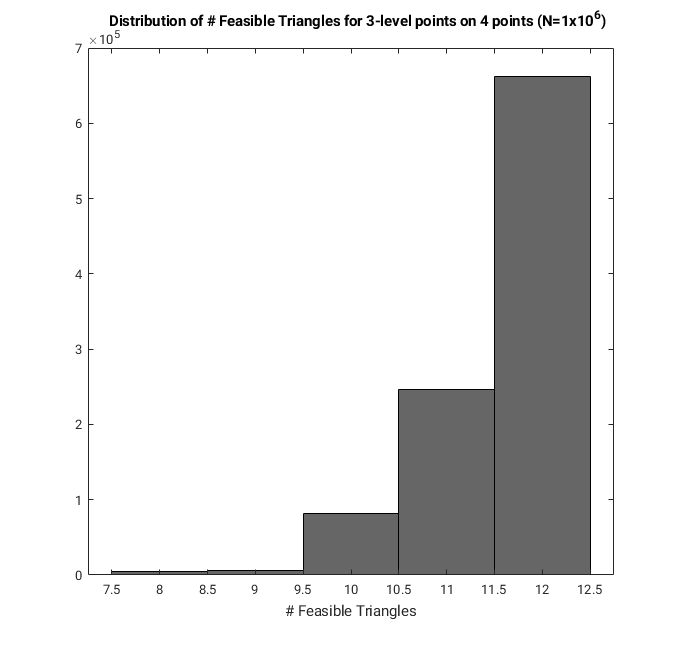
\includegraphics[width=0.45\textwidth]{figures/histogram_feasible_3_4.png}
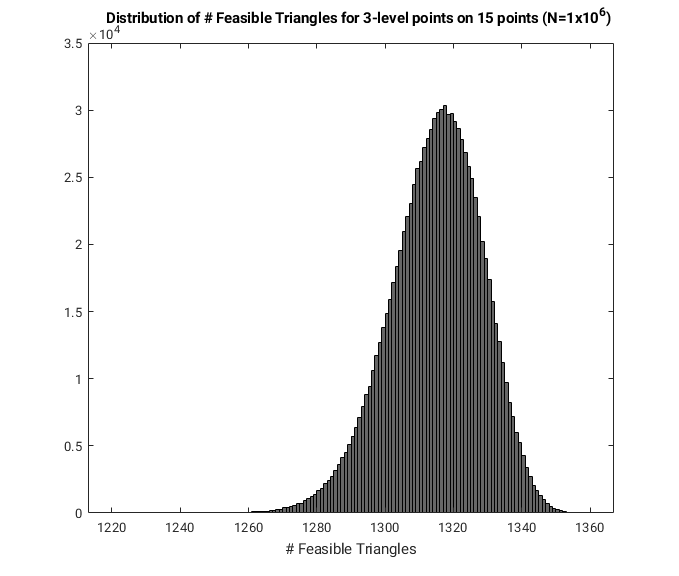
\includegraphics[width=0.45\textwidth]{figures/histogram_feasible_3_15.png}
\caption{Distribution of the number of feasible triangles among uniformly drawn $3$-level
points, $n=4$ (left) and $n=15$ (right).}
\label{fig:hist}
\end{figure}

\begin{figure}[htbp]
\centering
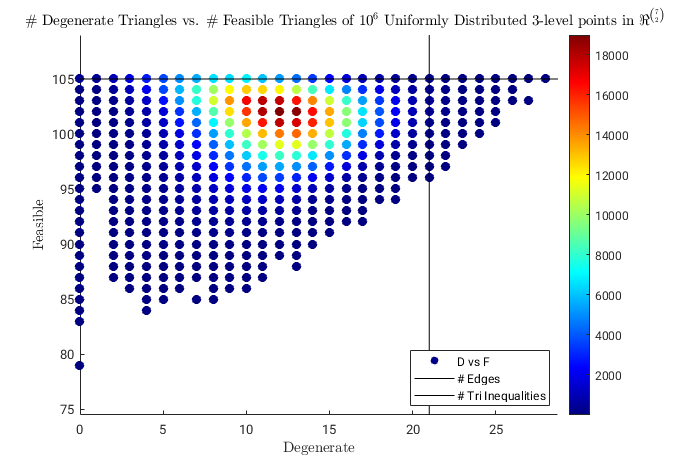
\includegraphics[width=0.45\textwidth]{figures/degen_feasible_3_7.png}
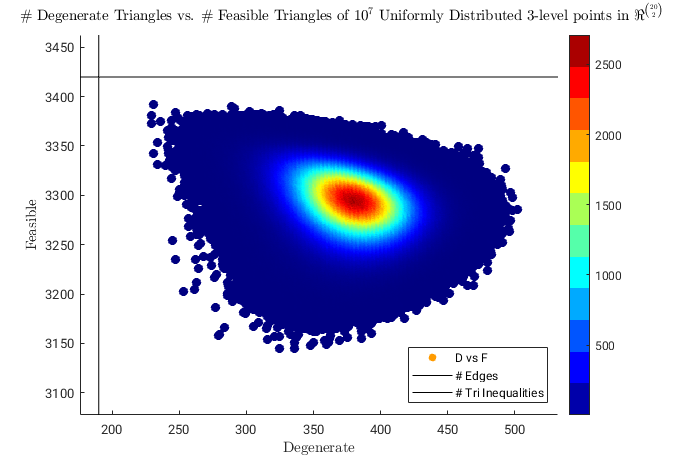
\includegraphics[width=0.45\textwidth]{figures/degen_feasible_3_20.png}
\caption{Degenerate versus feasible triangle counts for random $3$-level points, $n=7$
(left) and $n=20$ (right).}
\label{fig:degen}
\end{figure}

The bowtie family evades the tension by anchoring the degeneracies on a single unital stem.
Let
\[
\mathcal B^3_{n,1}=\bigl\{d\in I^3_n : \exists!\,I\in\mathcal E\ \text{with}\ d_I=1,\
\text{and every triangle containing }I\text{ is degenerate}\bigr\}.
\]
Every member is a metric---the infeasible pattern $(\tfrac13,\tfrac13,1)$ is excluded---and
the degenerate anchor lets the $(\tfrac13,\tfrac13,\tfrac23)$ degeneracies propagate.

%%%%%%%%%%%%%%%%%%%%%%%%%%%%%%%%%%%%%%%%%%%%%%%%%%%%%%%%%%
\section{Exterior angles}
\label{sec:angles}
%%%%%%%%%%%%%%%%%%%%%%%%%%%%%%%%%%%%%%%%%%%%%%%%%%%%%%%%%%

The probability that a vertex $d^*$ maximizes a uniformly random linear objective is
proportional to the volume of its dual cone met with the unit sphere: the exterior solid
polyhedral angle at $d^*$. Sampling random objectives therefore samples vertices by angle.

\begin{center}
\begin{tabular}{r|rrrr}
$n$ & partition & half-one & $\den\leq2$ & other\\
\hline
$5$ & $0.978$ & $0.000$ & $1.000$ & $0.000$\\
$8$ & $0.870$ & $0.007$ & $0.987$ & $0.013$\\
$10$ & $0.657$ & $0.003$ & $0.923$ & $0.077$\\
$14$ & $0.310$ & $0.040$ & $0.640$ & $0.360$\\
$18$ & $0.093$ & $0.107$ & $0.467$ & $0.533$\\
$20$ & $0.050$ & $0.275$ & $0.625$ & $0.375$\\
$24$ & $0.000$ & $0.530$ & $0.830$ & $0.170$\\
$32$ & $0.000$ & $0.967$ & $1.000$ & $0.000$\\
$40$ & $0.000$ & $1.000$ & $1.000$ & $0.000$
\end{tabular}
\end{center}

The half-one share is flat near zero through $n=12$, turns near $n=14$, crosses the
partition share near $n=18$, and reaches $1$ by $n=40$. An experiment confined to
$5\leq n\leq10$ sees only the flat initial segment, and would report no trend.

\begin{conjecture}[Gauss--Bonnet]\label{conj:gb}
The sum of the exterior solid polyhedral angles over the extreme half-one metrics on $n$
points converges, as $n\to\infty$, to the volume of the $\binom n2$-dimensional unit
sphere.
\end{conjecture}

The name records the analogy: the total exterior angle of a polytope is its whole sphere of
directions, and the conjecture asserts that the half-one vertices absorb all of that
curvature in the limit. The heuristic is that an extreme half-one metric lies on many more
supporting hyperplanes than extremality requires, having many degenerate triangles, and is
therefore a sharp corner with a large dual cone.

Three abundance statements should be kept apart. Theorem~\ref{thm:density} says half-one
metrics are almost all extreme; the table above says they win the angle competition from
about $n=20$; Conjecture~\ref{conj:gb} says they take all of it in the limit; and
Question~\ref{q:share} asks about their share of the vertices, where the evidence is
equivocal. The first is proved, the second observed, the third open, and the fourth may
have a different answer from the third.

A reduction worth recording: the total angle carried by non-half-one vertices is at most
the number of such vertices times the maximal angle at one of them, so any subexponential
bound on the maximal exterior angle at a non-half-one vertex, combined with a bound on
$|\ex(\bM_n)|$, would bear on Conjecture~\ref{conj:gb}. Proving it appears to require
estimating the hypergeometric series arising from the angular geometry of the
$e_{[i,j,k]}$-system of supporting hyperplanes.

%%%%%%%%%%%%%%%%%%%%%%%%%%%%%%%%%%%%%%%%%%%%%%%%%%%%%%%%%%
\section{Questions}
\label{sec:questions}
%%%%%%%%%%%%%%%%%%%%%%%%%%%%%%%%%%%%%%%%%%%%%%%%%%%%%%%%%%

\begin{question}\label{q:deficit}
Prove the upper bound matching Theorem~\ref{thm:twinbound}: that
$1-|\ex(\Ha_n)|/2^{\binom n2}=O\bigl(n^22^{-n}\bigr)$, establishing
Conjecture~\ref{conj:deficit}. What is required is a union bound over bipartite components
of $\Gamma_d$ with at least two nodes; the classification through $n=8$ shows every such
mode decaying at least at the rate $4^{-n}$ against the twin rate $2^{-n}$, but the number
of shapes grows and no uniform bound is proved.
\end{question}

Question~\ref{q:share} above asks for the growth of $|\ex(\bM_n)|$, and
Conjecture~\ref{conj:den12} for a denominator bound uniform in $n$. Two further questions:

\begin{question}
Is $|\ex(\bM_7)|$ computable by the method of Section~\ref{sec:census}? The denominator-$2$
sweep at $n=7$ is within reach and would extend Proposition~\ref{prop:pd} to $1309868$;
the full census requires denominators to $6$ and a better enumerator than exhaustive search
over grids.
\end{question}

\begin{question}
Theorem~\ref{thm:upperhalf} determines the vertices of $\bM_n$ in the closed upper
half-cube. The census shows the vertices below it organized by denominator; is there a
second value-set theorem there---a description of
$\ex(\bM_n)\cap[\tfrac13,1]^{\binom n2}$, say, where degenerate triangles of patterns
other than $\tfrac12+\tfrac12=1$ first become available?
\end{question}

\begin{thebibliography}{9}

\bibitem{Avis80}
D.~Avis, On the extreme rays of the metric cone,
\textit{Canad.\ J.\ Math.}~\textbf{32} (1980), no.~1, 126--144.

\bibitem{Bandelt92}
H.-J.~Bandelt and A.W.M.~Dress, A canonical decomposition theory for metrics on a finite
set, \textit{Adv.\ Math.}~\textbf{92} (1992), no.~1, 47--105.

\bibitem{Berend10}
D.~Berend and T.~Tassa, Improved bounds on Bell numbers and on moments of sums of random
variables, \textit{Probab.\ Math.\ Statist.}~\textbf{30} (2010), no.~2, 185--205.

\bibitem{Deza97}
M.M.~Deza and M.~Laurent, \textit{Geometry of Cuts and Metrics}, Springer-Verlag,
Berlin--Heidelberg, 1997.

\bibitem{FK-cone}
D.V.~Feldman and E.R.~Kehoe, Extreme rays of the metric cone and the metric body: bowtie
metrics and half-one extremality, companion paper; the results quoted here also appear as
\cite[Ch.~2--4]{Kehoe19}.

\bibitem{Kehoe19}
E.R.~Kehoe, \textit{Pseudometrics, the Complex of Ultrametrics, and Iterated Cycle
Structures}, Ph.D.\ dissertation, University of New Hampshire, 2019.
\url{https://scholars.unh.edu/dissertation/2451}

\bibitem{McMullen70}
P.~McMullen, The maximum numbers of faces of a convex polytope,
\textit{Mathematika}~\textbf{17} (1970), 179--184.

\bibitem{Koolen00}
J.~Koolen, V.~Moulton, and U.~T\"onges, A classification of the six-point prime metrics,
\textit{European J.\ Combin.}~\textbf{21} (2000), no.~6, 815--829.

\bibitem{Spencer68}
J.~Spencer, Maximal consistent families of triples, \textit{J.\ Combinatorial
Theory}~\textbf{5} (1968), 1--8.

\end{thebibliography}

\end{document}
